\section*{Figure Legends}
\label{figures}

\subsubsection*{Figure~\ref{fig:chondrocyte-model}.}
An illustration summarising the various channels considered in the
current electrophysiological model of the chondrocyte.

\subsubsection*{Figure~\ref{fig:potassium-currents}.}
Potassium currents which are fit to experimental values (in red) from
\citet{Clarketal2011}. The external concentrations correspond to the
experimental conditions: \Ko = 5~mM, \Nao = 140~mM, \Cao = 2~mM, pH =
7.4, except for $I_{K_{\mathrm{2\; pore}}}$, where \Ko = 145~mM, pH = 8.5.

\subsubsection*{Figure~\ref{fig:other-currents}.}
V-I relations for the other currents. These are not fit to
experimental data, but used to tune simulation results.

\subsubsection*{Figure~\ref{fig:overall-behaviour}.}
Overall behaviour of the model when voltage is ramped from -130~mV to
+90~mV in 1~s. It validates well with respect to experimental data
(red) from \citet{Clarketal2011}.

\subsubsection*{Figure~\ref{fig:concentrations}.}
Time-evolution of the concentrations over 1800~s to show that the
initial conditions we have chosen for the model were at steady
state. The initial conditions for the concentrations used in the
computations were \Nai = 2.814~mM, \Ki = 121.59~mM, \Cai =
2.371e-06~mM, \Hi = 6.188e-10~mM, \Cli = 13.209~mM.

\subsection*{Figure~\ref{fig:I_K_2pore-rmp}}
When the amount of $I_{K_{\mathrm{2\; pore}}}$ is varied from 100\% to
0\% (by blocking with increasing amounts of BUP), the RMP
increases. These simulations were carried out at two different values
of external concentrations \Ko = 5~mM and \Ko = 25~mM and validates
well with respect to experimental data
\citep[Fig. 8B]{Clarketal2011}.

\subsubsection*{Figure~\ref{fig:K_o-rmp}}
Evolution of the resting membrane potential with varying external
potassium concentration. Note that while it is slightly more positive
than experiments, it matches the qualitative behaviour quite
closely \citep{Clarketal2011}.

\clearpage
\setlength{\textwidth}{18cm}
\setlength{\oddsidemargin}{0in}
\setlength{\evensidemargin}{0in}

\begin{landscape}
\begin{figure}
  \centering
  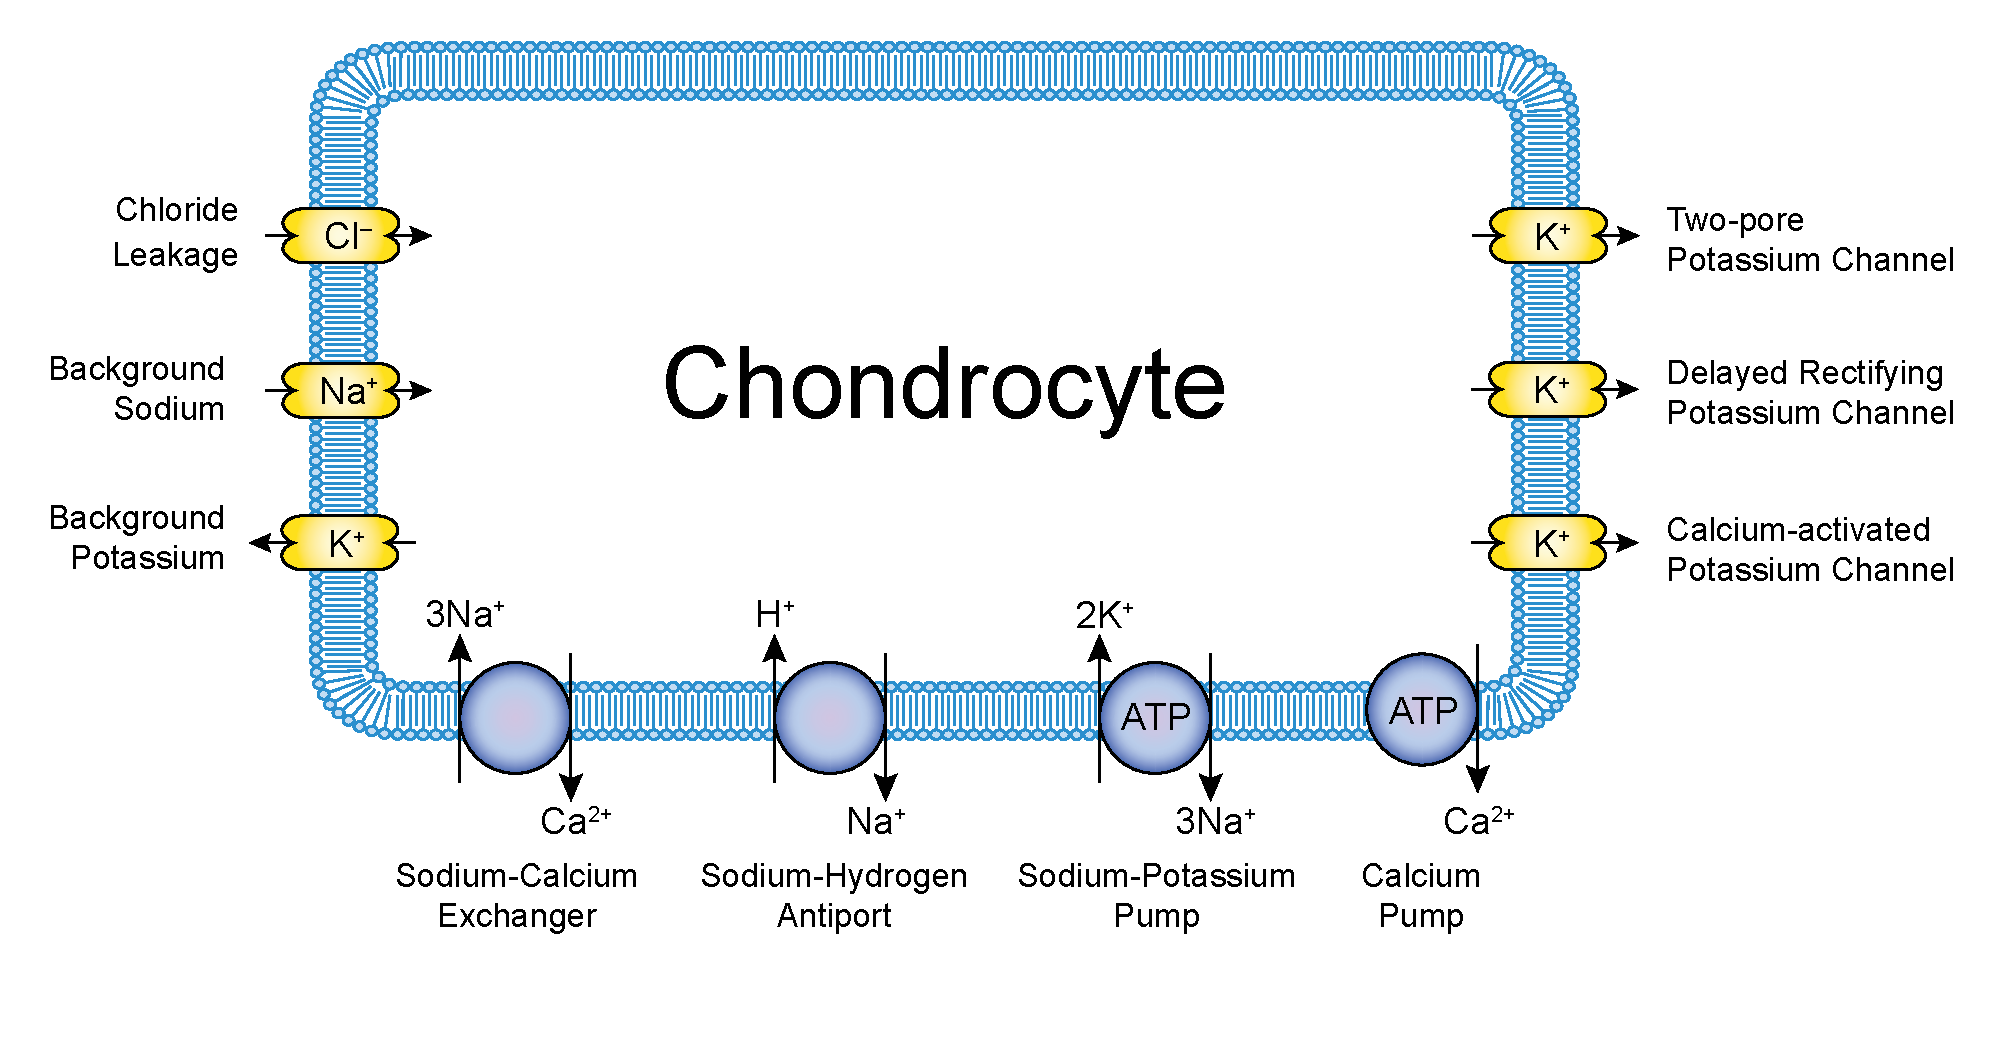
\includegraphics[width=\textwidth]
  {../images/pdf/chondrocyte-model-cellml}
  \caption{}
  \label{fig:chondrocyte-model}
\end{figure}
\end{landscape}

\clearpage
\begin{landscape}
\begin{figure}
  \centering
  \subfloat{\includegraphics[width=0.5\textwidth]
    {../results/pdf/20120803/V-I_K_2pore}}
  \subfloat{\includegraphics[width=0.5\textwidth]
    {../results/pdf/20120803/V-I_K_Ca_act}}\\
  \subfloat{\includegraphics[width=0.5\textwidth]
    {../results/pdf/20120803/V-I_K_ur}}
  \subfloat{\includegraphics[width=0.5\textwidth]
    {../results/pdf/20120803/t-I_K_ur}}
  \caption{}
  \label{fig:potassium-currents}
\end{figure}
\end{landscape}

\clearpage
\begin{landscape}
\begin{figure}
  \centering
  \subfloat{\includegraphics[width=0.5\textwidth]
    {../results/pdf/20120803/V-I_Na_b}}
  \subfloat{\includegraphics[width=0.5\textwidth]
    {../results/pdf/20120803/V-I_NaCa}}\\
  \subfloat{\includegraphics[width=0.5\textwidth]
    {../results/pdf/20120803/V-I_NaK}}
  \subfloat{\hspace{0.5\textwidth}}
  \caption{}
  \label{fig:other-currents}
\end{figure}
\end{landscape}

\clearpage
\begin{landscape}
\begin{figure}
  \centering
  \subfloat{\includegraphics[width=0.5\textwidth]
    {../results/pdf/20120803/t-v}}
  \subfloat{\includegraphics[width=0.5\textwidth]
    {../results/pdf/20120803/V-I_i_by_Cm}}\\
  \subfloat{\includegraphics[width=0.5\textwidth]
    {../results/pdf/20120803/t-I_i}}
  \subfloat{\hspace{0.5\textwidth}}
  \caption{}
  \label{fig:overall-behaviour}
\end{figure}
\end{landscape}

\clearpage
\begin{figure}
  \centering
  \subfloat{\includegraphics[width=0.50\textwidth]
    {../results/pdf/20120803/t-Na_i}}
  \subfloat{\includegraphics[width=0.50\textwidth]
    {../results/pdf/20120803/t-K_i}}\\
  \subfloat{\includegraphics[width=0.50\textwidth]
    {../results/pdf/20120803/t-Ca_i}}
  \subfloat{\includegraphics[width=0.50\textwidth]
    {../results/pdf/20120803/t-H_i}}\\
\subfloat{\includegraphics[width=0.50\textwidth]
  {../results/pdf/20120803/t-Cl_i}}
  \subfloat{\hspace{0.50\textwidth}}\\
  \caption{}
  \label{fig:concentrations}
\end{figure}

\clearpage
\begin{landscape}
\begin{figure}
  \centering
  \includegraphics[width=1.0\textwidth]
    {../results/pdf/20120803/I_K_2pore_vs_RMP}
  \caption{}
  \label{fig:I_K_2pore-rmp}
\end{figure}
\end{landscape}

\clearpage
\begin{landscape}
\begin{figure}
  \centering
  \includegraphics[width=1.0\textwidth]
    {../results/pdf/20120803/K_o_vs_RMP}
  \caption{}
  \label{fig:K_o-rmp}
\end{figure}
\end{landscape}

% Local Variables:
% TeX-master: "chondrocyte-model"
% mode: latex
% mode: flyspell
% End:
